\chapter{Direct reinforcement learning of decision tree policies for classification tasks}\label{sec:pomdp-classif}
In this section, we show that for a special class of POIBMDPs~\ref{def:poibmdp}, reinforcement learning~\ref{sec:rl} can retrieve optimal deterministic partially observable policies w.r.t to the interpretable RL objective (\ref{def:revised}), i.e. we can do direct decision tree policy learning for MDPs.
This class of POIBMDPs are those for which base MDPs have uniform transitions, i.e. $T(\boldsymbol{s}, a, \boldsymbol{s}') = \frac{1}{|S|}$ (cf. definitions~\ref{def:mdp} and~\ref{def:ibmdp}).
The supervised learning objective (\ref{def:sl}) can be re-formulated in terms of the RL objective (\ref{def:mdp-obj}) and MDPs with such uniform transitions.
Indeed a supervised learning task can be formulated as maximizing the RL objective in an MDP where, actions are class (or target) labels, states are training data, the reward at every step is 1 if the correct label was predicted and 0 otherwise, and the transitions are uniform: the next state is given by uniformly sampling a new training datum. 
This implies that learning deterministic partially observable policies in POIBMDPs where the base MDP encodes a supervised learning task is equivalent to doing decision tree induction to optimize the supervised learning objective~\ref{def:sl}.
If RL does work for such fully observable POIBMDPs, this would mean that: 1. the difficulty of direct learning of decision tree policies for \textit{any} MDP using POIMDPs, exhibited in the previous chapters, is most likely due to the partial observability, and 2., it means that we can design new decision tree induction algorithms for~\ref{def:sl} by solving MDPs.

Let us show that, POIBMDPs~\ref{def:poibmdp} associated with MDPs encoding supervised learning tasks, are in fact MDPs~\ref{def:mdp}.

Let us define such supervised learning MDPs in the context of a classification task (this definition extends trivially to regression tasks).
\begin{definition}[Classification Markov decision process]\label{def:cmdp}
    Given a set of $N$ examples denoted $\mathcal{E} = {\{(x_i, y_i)\}}_{i=1}^N$ where each datum $x_i$ is described by a set of $p$ features and $y_i \in \mathbb{Z}^m$ is the label associated with $x_i$, a classification Markov decision Process is an MDP $\langle S, A, R, T, T_0 \rangle$~\ref{def:mdp} where:
    \begin{itemize}
        \item the state space is $S={\{\boldsymbol{x}_i\}}_{i=1}^N$, the set of training data features
        \item the action space is $A=\mathbb{Z}^m$, the set of unique labels
        \item the reward function is $R:S\times A \rightarrow \{0, 1\}$ with $R(\boldsymbol{s}=\boldsymbol{x}_i, a) = 1_{a=y_i}$
        \item the transition function is $T:S\times A \rightarrow \Delta(S)$ with $T(\boldsymbol{s}, a, \boldsymbol{s}') = \frac{1}{N} \quad \forall \boldsymbol{s}, a, \boldsymbol{s}'$
        \item the initial distribution is $T_0(\boldsymbol{s}_0 = \boldsymbol{s}) = \frac{1}{N}$
    \end{itemize}
\end{definition}

One can be convinced that policies that maximize the RL objective~\ref{def:mdp-obj} in classification MDPs are classifiers that maximize the prediction accuracy because $\sum_{i=1}^N 1_{\pi(\boldsymbol{x}_i)=y_i} = \sum_{i=1}^N R(x_i, \pi(\boldsymbol{x}_i))$.
We defer the formal proof in the next part of the manuscript in which we extensively study supervised learning problems.

In figure~\ref{example:cmdp} we give an example of such classification MDP with 4 data in the training set and 2 classes:
\begin{align*}
    \mathcal{X} &= \{(0.5, 0.5), (0.5, 1.5), (1.5, 1.5), (1.5, 0.5)\}\\
    y &= \{0, 0, 1, 1\} 
\end{align*}

\begin{figure}
    \centering
    \begin{tikzpicture}[
        decision/.style={circle, draw, thick, fill=blue!20, text width=2.5em, text centered, minimum height=2.5em, font=\small},
        leaf/.style={rectangle, draw, thick, fill=green!20, text width=2em, text centered, rounded corners, minimum height=2em, font=\small},
        edge_label/.style={font=\footnotesize, midway}
    ]
        % Tree 4: if x <= 0.5 move right else move left
        \node[decision] (tree4_root) at (8,2) {$x \leq 1$};
        \node[rectangle, draw, thick, fill=green!40, text width=2em, text centered, rounded corners, minimum height=2em, font=\small] (tree4_right) at (7,0) {};
        \node[rectangle, draw, thick, fill=red!40, text width=2em, text centered, rounded corners, minimum height=2em, font=\small] (tree4_left) at (9,0);
        \draw[->] (tree4_root) -- (tree4_right) node[edge_label, above left] {True};
        \draw[->] (tree4_root) -- (tree4_left) node[edge_label, above right] {False};
        \tikzstyle{grid}=[draw, thick, fill=gray!10]
        
        % Draw grid
        \draw[fill=green!40] (0, 0) rectangle (1,2);
        \draw[fill=red!40] (1, 0) rectangle (2,2);

        \draw[grid] (0,0) grid (2,2);
        
        % Add axes
        \draw[thick, ->] (0,0) -- (2.5,0) node[right] {$x$};
        \draw[thick, ->] (0,0) -- (0,2.5) node[above] {$y$};
        
        % Add tick marks and labels
        \foreach \x in {0,1,2} {
            \draw[thick] (\x,0) -- (\x,-0.1) node[below] {$\x$};
        }
        \foreach \y in {0,1,2} {
            \draw[thick] (0,\y) -- (-0.1,\y) node[left] {$\y$};
        }

        \node at (0.5,0.5) {$\boldsymbol{s}_0$};
        \node at (1.5,0.5) {$\boldsymbol{s}_g$};
        \node at (1.5,1.5) {$\boldsymbol{s}_2$};
        \node at (0.5,1.5) {$\boldsymbol{s}_1$};

    \end{tikzpicture}
    \caption{Classification MDP optimal actions. In this classification MDP, there are four data to which to assign either a green or red label.
    On the right, there is the unique optimal depth-1 tree for this particular classification MDP. This depth-1 tree also maximizes the accuracy on the corresponding classification task.}\label{example:cmdp}
    \end{figure}

Now let us show that associated POIBMDPs are in fact MDPs. We show this by construction.

\begin{definition}[Classification POIBMDP]\label{def:cpoibmdp}
    Given a classification MDP $\langle {\{\boldsymbol{x}_i\}}_{i=1}^N, \mathbb{Z}^m, R, T, T_0 \rangle$ (\ref{def:cmdp}), and an associated POIBMDP $\langle S, O, A, A_{info}, R, \zeta, T_{info}, T, T_0\rangle$ (\ref{def:poibmdp}), a classification POIBMDP is an MDP (\ref{def:mdp}):
    \begin{align*}
        \langle \overbrace{O}^{\text{State space}}, \underbrace{\mathbb{Z}^m, A_{info}}_{\text{Action space}}, \overbrace{R, \zeta}^{\text{Reward function}}, \underbrace{\mathcal{P}, \mathcal{P}_0}_{\text{Transition kernels}} \rangle
    \end{align*}
    \begin{itemize}
        \item $O$ is the set of possible observations in $[L_1, U_1] \times \dots \times [L_p, U_p] \times [L_1, U_1] \ times \dots \times [L_p, U_p] $ where $L_j$ is the minimum value of feature $j$ over all data $x_i$ and $U_j$ the maximum
        \item $\mathbb{Z}^m \cup A_{info}$ is action space: actions can be label assignments in $\mathbb{Z}^m$ or bounds refinement in $A_{info}$
        \item The reward for assigning label $a\in \mathbb{Z}^m$ when observing some observation $\boldsymbol{o}=(L'_1, U'_1, \dots, L'_p, U'_p)$ is the proportion of training data satistifying the bounds and having label $a$: $R(o, a) = \frac{|\{x_i: L'_j \leq x_{ij} \leq U'_j \forall i,j \} \cap \{\boldsymbol{x}_i: y_i = a \forall i \}|}{|\{\boldsymbol{x}_i: L'_j \leq x_{ij} \leq U'_j \forall i,j \}|}$. 
        The reward for taking an information gathering action that refines bounds is $\zeta$
        \item The transition kernel is $\mathcal{P}:O \times (\mathbb{Z}^m \cup A_{info}) \rightarrow \Delta O$ where:
        \begin{itemize}
            \item For $a \in \mathbb{Z}^m$: $\mathcal{P}(\boldsymbol{o}, a, (L_1, U_1, \dots, L_p, U_p)) = 1$ (reset to full bounds)
            \item For $a = (k, v) \in A_{info}$: from $\boldsymbol{o}=(L'_1, U'_1, \dots, L'_p, U'_p)$, the MDP will transit to $\boldsymbol{o}_{left} = (L'_1, U'_1, \dots, L_k, v, dots, L'_p, U'_p)$ (resp. $\boldsymbol{o}_{right} = (L'_1, U'_1, \dots, U'_k, v, dots, L'_p, U'_p)$) with probability $\frac{|\{\boldsymbol{x}_i: L'_j \leq x_{ij} \leq U'_j \forall j \land x_{ik} \leq v\}|}{|\{\boldsymbol{x}_i: L'_j \leq x_{ij} \leq U'_j \forall j\}|}$ (resp. $\frac{|\{\boldsymbol{x}_i: L'_j \leq x_{ij} \leq U'_j \forall j \land x_{ik} > v\}|}{|\{\boldsymbol{x}_i: L'_j \leq x_{ij} \leq U'_j \forall j\}|}$)
        \end{itemize}
    \end{itemize}
\end{definition}

Those classification POIBMDPs are essentially MDPs with stochastic transitions.
It means that deterministic partially observable policies (\ref{def:po-policy}) $O:\rightarrow A\cup A_{info}$ are in fact Markovian policy for those classification POIBMDPs.
More importantly, it means that, for a given $\gamma$ and $\zeta$, if we were to know the whole POIBMDP model, we could use planning, e.g. value iteration (\ref{alg:value-iteration}), to compute \textit{optimal} decision tree policies.
Similarly, standard RL algorithms like Q-learning (\ref{sec:rl}) should work as well as for any MDP to retrieve optimal decision tree policies.

This exactly what we check next.
We use the exact the same framework to learn decision tree policies as summarized in figure~\ref{fig:summary-rl} except that now, the base MDP is a classification task and not a sequential decision making task.

\section{How well can RL baselines learn in classification POIBMDPs?}
Similarly to the previous chapter, we are interested in a very simple classification POIBMDP.
We study classification POIBMDPs associated with the example classification MDP from figure~\ref{example:cmdp}.

We construct classification POIBMDPs with $\gamma=0.99$, 200 values of $\zeta \in [0,1]$ and IGAs $x\leq 1$ and $y\leq 1$.
Since classification POIBMDPs are MDPs, we do not need to analyze asymmetric RL and JSJ baselines like in the previous chapter (aglorithms~\ref{alg:asymqlearning},~\ref{alg:asymsarsa}, and~\ref{alg:jsj}).

\begin{figure}
    \centering
    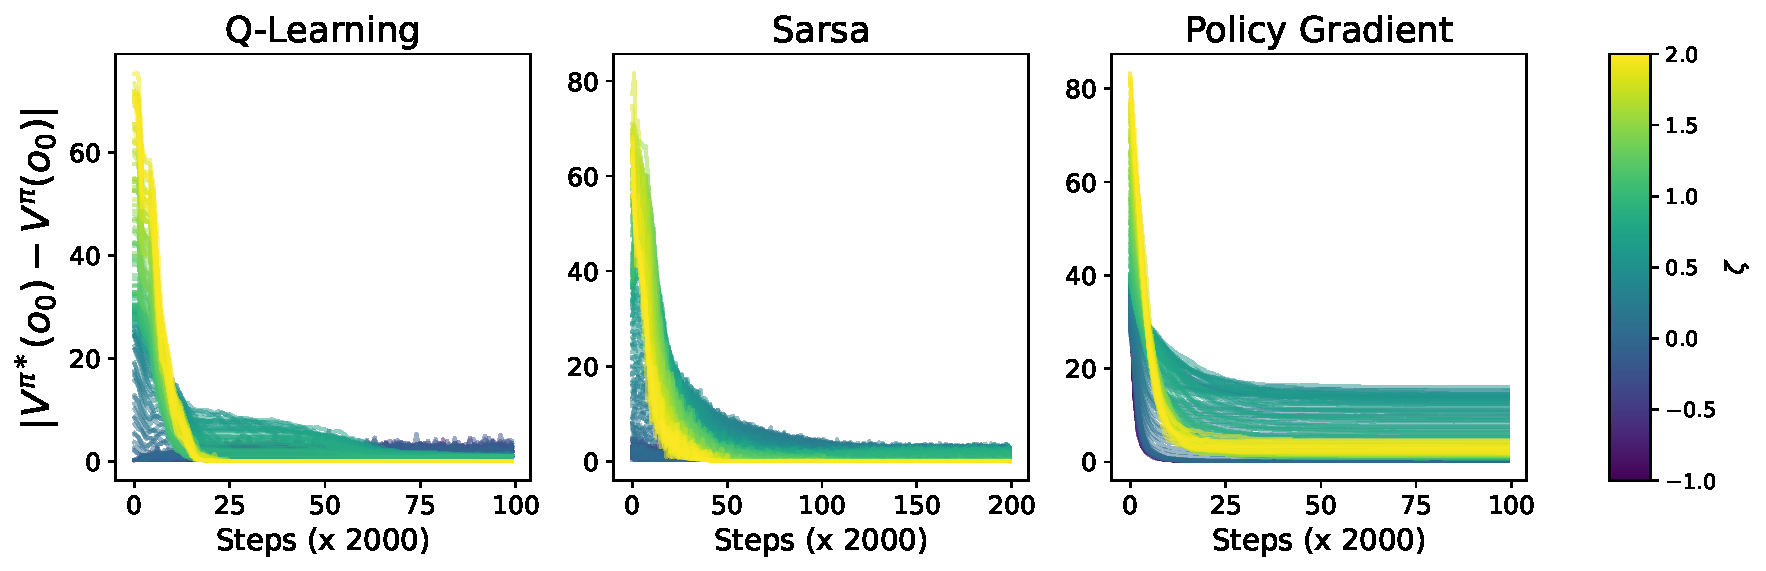
\includegraphics[width=1\textwidth]{images/images_part1/learning_curves_classif.pdf}
    \caption{We reproduce the same plot as in figure~\ref{fig:rl-poibmdp} for classification POIBMDPs. Each individual curve is the sub-optimality gap of the learned policy during training averaged over 100 runs for a single $\zeta$ value.}\label{fig:rl-classif-poibmdp}
\end{figure}

\begin{figure}
    \centering
    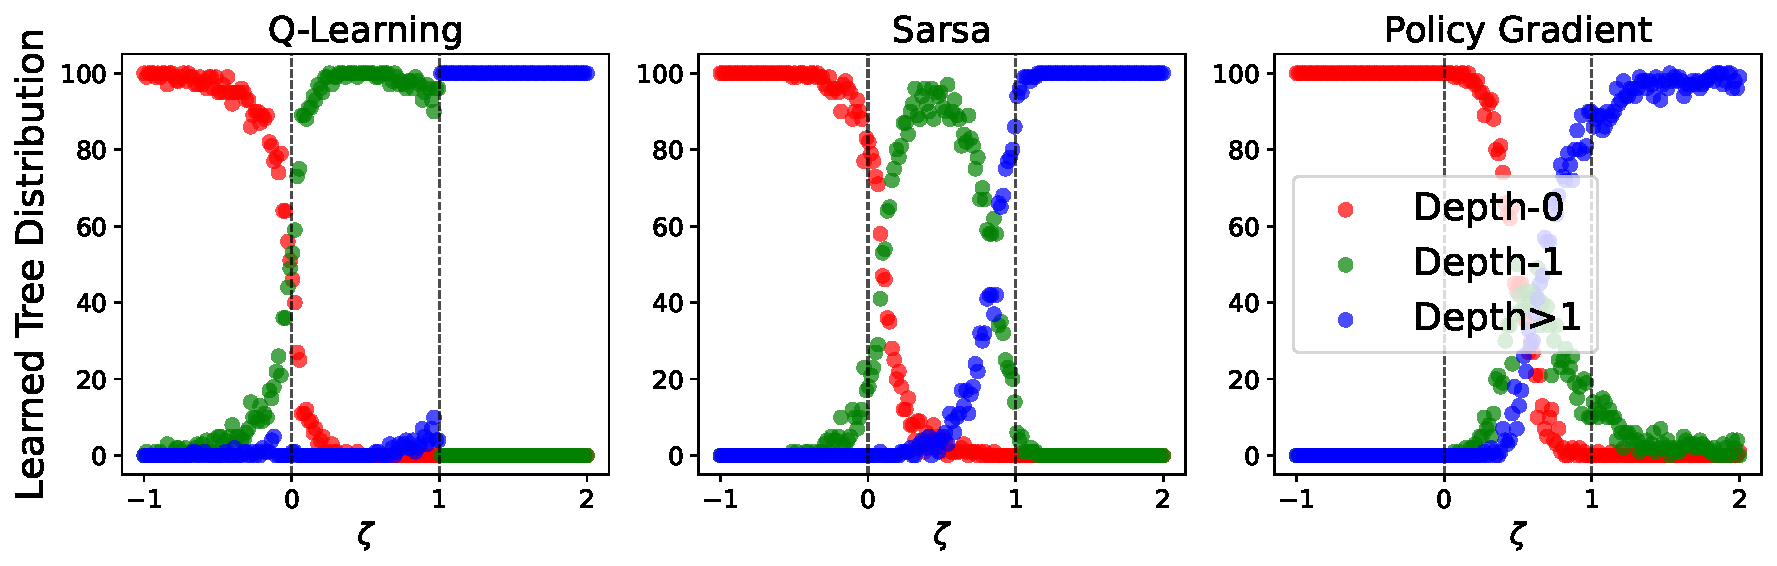
\includegraphics[width=1\textwidth]{images/images_part1/tree_distributions_classif.pdf}
    \caption{We reproduce the same plot as in figure~\ref{fig:dt-distrib-poibmdp} for classification POIBMDPs. Each colored dot is the number of final learned trees with a specific structure for a given $\zeta$.}\label{fig:tree-distrib-classif-poibmdp}
\end{figure}

Fortunately this time, compared to general POIBMDPs, RL can be used to retrieve optimal deterministic partially observable policies $O:\rightarrow A\cup A_{info}$ w.r.t. the interpretable RL objective (\ref{def:revised}) in classification POIBMDPs.
Such policies are equivalent to decision tree classifiers.
We observe on figure~\ref{fig:rl-classif-poibmdp} that both Q-learning and Sarsa consistently minimize the sub-optimality gap indepedently of the interpretability-performance trade-off $\zeta$. 
Hence they are able to retrieve the optimal depth-1 decision tree classifier (figure~\ref{example:cmdp}) most of the time in the optimality range $\zeta\in ]0, 1[$ (cf. figure~\ref{fig:tree-distrib-classif-poibmdp}).


\section{Conclusion}\label{sec:ccl-pomdp}
In this part of the manuscript we were interested in algorithms that can learn decision tree policies that optimize some trade-off of interpretability and performance w.r.t. the RL objective~\ref{def:mdp-obj} in MDPs.
In particular, using the framework of Topin et. al.~\cite{topin2021iterative}, we were able to explicitly write an interpretable RL objective function~\ref{def:irl}.

In chapter~\ref{sec:topin}, we compared the algorithms proposed in~\cite{topin2021iterative} that directly optimize this objective, to imitation learning algorithms that only solve a proxy problem.
While those direct RL algorithms are able to \textit{learn}, i.e. find better and better solutions with time (cf. figures~\ref{fig:res-dqn} and~\ref{fig:res-ppo}), the decision tree policies returned perform worse in average than imitated decision trees w.r.t. to the RL objective of interest (cf. figure~\ref{fig:ppo-trees}) for similar number of nodes and depth.

We further analyzed the failure mode of direct learning of decision tree policies by making connexions with POMDPs~\cite{POMDP,chap2}.
In chapter~\ref{sec:pomdp}, we showed that learning decision tree policies for MDPs could be explicitly formulated as learning a deterministic partially observable (also known as memoryless or reactive) policy in a specific POMDP that we called POIBMDP~\ref{def:poibmdp}.
We showed that both RL and asymmetric RL, a class of algorithms specifically designed for POMDPs~\cite{baisero-ppo,baisero-dqn}, were unable to consistently retrieve an optimal depth-1 decision tree policies for a very small grid world MDP when using the POIBMDP framework.
In particular, we compared, in a very controlled experiment, the success rates of the same learning algorithms when seeking standard Markovian policies versus partially observable policies in decision processes that shared the same transitions and rewards (cf. section~\ref{sec:how-diff}).
We demonstrated on figure~\ref{fig:po-vs-ib} that introducing partial observability greatly reduced the success rates (we also observed this implicitly on figures~\ref{fig:res-dqn} and~\ref{fig:res-ppo}).  

Finally, in this chapter we showed that using RL to optimize the interpretable RL objective in fully observable POIBMDPs, i.e. POIBMDPs that are just MDPs, could retrieve optimal decision tree policies (cf. figures~\ref{fig:rl-classif-poibmdp} and~\ref{fig:tree-distrib-classif-poibmdp}) adding new evidence that direct interpretable RL is difficult because it involves POMDPs.

This class of fully observable POIBMDPs contains the decision tree induction problem for supervised learning tasks~\ref{def:sl} (cf. Defs.~\ref{def:cmdp} and~\ref{def:cpoibmdp}).
This sparks the question: what kind of decision tree induction algorithm can we get using the MDP formalism?
This exactly what we study in the next part of this manuscript.

Those few chapters raise other interesting questions.
First, while we focused on non-parametric tree learning with the promise that RL algorithms could naturally trade off interpretability and performances, parametric tree learning should be studied since it does not have this partial observability component.
Since existing RL for parametric decision tree policies \cite{silva,vos2024optimizinginterpretabledecisiontree,sympol} require to re-train a policy entirely for each desired level interpretability, i.e. each unique tree structure, future research in this direction should focus on algorithms for parametric tree policies that can re-use samples from one tree learning to train a different tree structure more efficiently.
This would reduce the required quantity of a priori knowledge on the decision tree policy structure mentioned in section~\ref{related-work-pomdp}.

Attempting to overcome the partial observability challenges highlighted so far seems like a bad research avenue.
Indeed, while algorithms tailored specifically for the problem of learning deterministic partially observable policies for POIBMDPs might exist, we clearly saw that imitation learning was in practice a good alternative to direct interpretable reinforcement learning.
And even if the former makes the promise of naturally trading off interpretability and performances, some limitations that we did not cover still exist such as how to choose good candidates information gathering actions or simply how to choose $\zeta$ for a target interpretability-performance trade-off.
